% Provenance (never printed): old premiere S material on the oceanic lithosphere
% (ophiolite-type layering, peridotite and gabbro, partial melting by decompression
% at the ridge, hydrothermalism, cooling and subsidence of the lithosphere with
% age); see sources/book2/PROVENANCE.md. Melting from figdata/grade-11/
% ridge_melting.py (adiabat and Hirschmann solidus), depth against age from
% depth_age.py (ETOPO1 and the Seton 2020 age grid). Partial melting is re-founded
% in Year 2 (mantle-melting); fault is Book 1's (g7), normal fault is defined here.
\chapter{Les dorsales océaniques et la lithosphère océanique}\label{ch:g11:ocean-ridges}

En février 1977, un traîneau photographique remorqué à 2500 mètres de
profondeur au-dessus du rift des Galápagos, dans le Pacifique Est,
photographiait image après image la lave noire et nue de la dorsale. Puis
son thermomètre enregistra une légère hausse de la température de l'eau, et
sur les photographies la lave était couverte de centaines de palourdes
blanches. Quelques jours plus tard, le submersible \emph{Alvin} emmena deux
géologues sur place~: une eau tiède et miroitante sortait des fissures de
la lave, et tout autour vivaient des palourdes longues comme un avant-bras,
des moules et des crabes blancs~; lors d'une plongée ultérieure, des vers
tubicoles au panache rouge. Personne ne s'attendait à trouver de la vie à
cet endroit~: aucun biologiste n'était donc à bord. Ce chapitre explique ce
que les géologues avaient trouvé~: comment le fond océanique se forme aux
dorsales, pourquoi il y est chaud, et ce qu'il devient en s'en éloignant.
% ledger: whoi:alvin-1977

\begin{recall}
Aux dorsales se forme un nouveau fond océanique, qui s'éloigne des deux
côtés, si bien que son âge augmente avec la distance à l'axe~; les dorsales
forment un système long d'environ \qty{65000}{km}, avec une vallée de rift
le long des dorsales lentes et une crête lisse le long des dorsales rapides
(\cref{ch:g11:drift-to-spreading}). Les plaques s'écartent de part et
d'autre d'une dorsale de quelques centimètres par an, plus vite de part et
d'autre de la dorsale du Pacifique Est que de part et d'autre de la dorsale
médio-atlantique (\cref{ch:g11:plate-motions}). La \omterm{def:g11:lithosphere-asthenosphere:lithosphere}{lithosphère} est
l'enveloppe externe rigide, l'\omterm{def:g11:lithosphere-asthenosphere:lithosphere}{asthénosphère} située dessous s'écoule~; la
température de l'\omterm{def:g11:lithosphere-asthenosphere:lithosphere}{asthénosphère} n'augmente que d'environ \qty{0.45}{\celsius}
par kilomètre de profondeur, et la température de fusion de la roche du
manteau augmente avec la profondeur
(\cref{ch:g11:lithosphere-asthenosphere}). Le magma est de la roche fondue
sous la surface, le basalte la roche sombre que forme la lave en
refroidissant, et une faille une cassure le long de laquelle des roches se
sont déplacées (livre~1, années~6 et~7).
\end{recall}
% ledger: noaa:ridge, katsura10:adiabat, hirschmann:solidus

\section{La lithosphère océanique}

Deux roches rares à la surface des continents forment l'essentiel de la
\omterm{def:g11:ocean-ridges:oceanic-lithosphere}{lithosphère océanique}.

\begin{definition}[Péridotite]\label{def:g11:ocean-ridges:peridotite}
La \emph{péridotite}\index{peridotite@péridotite} est une roche sombre, à
gros grains, faite surtout d'un minéral, l'olivine, avec un peu de pyroxène.
Elle est en général verte et dense. On pense qu'une grande partie du manteau
terrestre est faite de péridotite.
\end{definition}

\begin{definition}[Gabbro]\label{def:g11:ocean-ridges:gabbro}
Le \emph{gabbro}\index{gabbro} est une roche magmatique sombre, à gros
grains, faite surtout de feldspath plagioclase et de pyroxène. Il a la même
composition que le basalte, mais il a cristallisé lentement, en profondeur,
ce qui a laissé à ses cristaux le temps de grandir. C'est la roche la plus
abondante de la \omterm{def:g11:ocean-ridges:oceanic-lithosphere}{croûte océanique} profonde.
\end{definition}
% ledger: geo:peridotite, geo:gabbro

Les minéraux cités ici, l'olivine, le pyroxène et le feldspath, sont décrits
au \cref{ch:g11:minerals}.

\begin{omfigure}
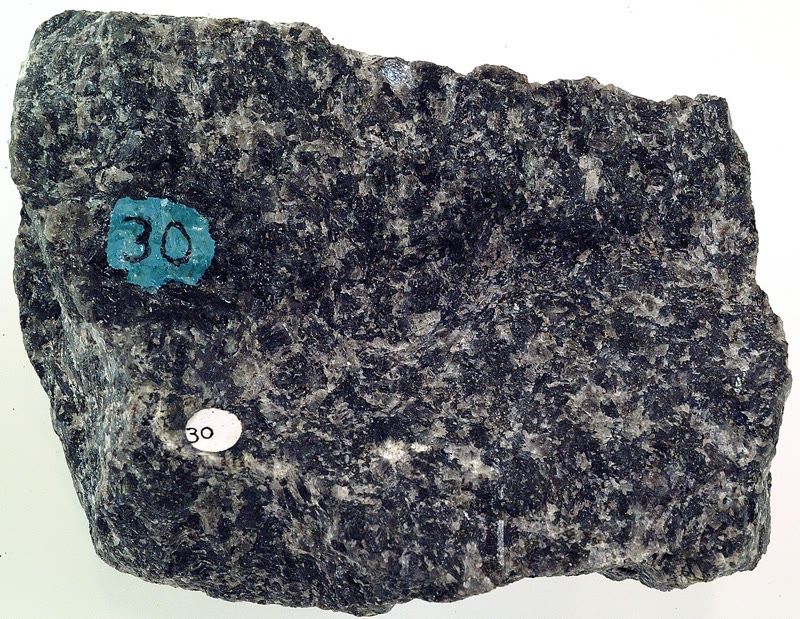
\includegraphics[height=4.2cm]{images/book2/g11-geodil-gabbro.jpg}\hspace{0.03\linewidth}%
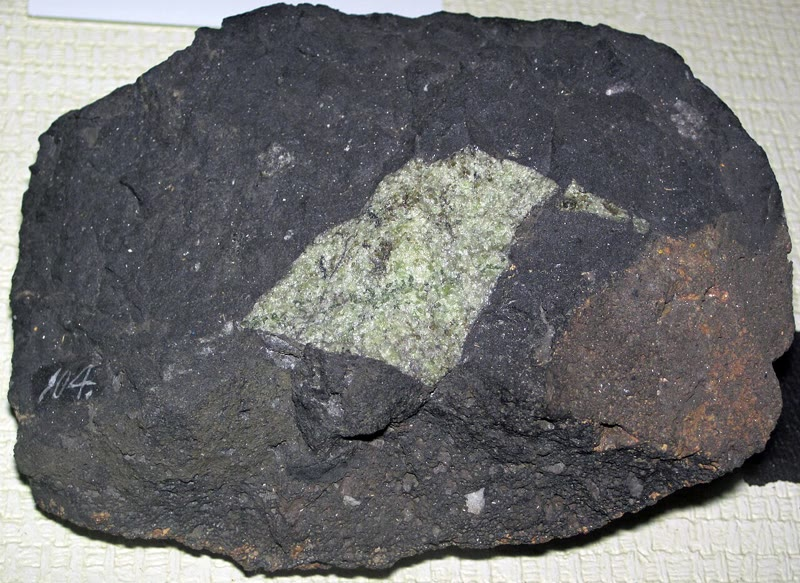
\includegraphics[height=4.2cm]{images/book2/g11-stjohn-peridotite.jpg}

{\small À gauche~: un \omterm{def:g11:ocean-ridges:gabbro}{gabbro}, large de \qty{9}{cm}, dont les cristaux sombres
de pyroxène et clairs de feldspath sont assez grands pour être vus~;
photographie Darla Sondrol (CC0). À droite~: un fragment de \omterm{def:g11:ocean-ridges:peridotite}{péridotite} verte
venue du manteau, remonté dans la lave basaltique noire d'un volcan de
l'Arizona~; photographie James St.~John (CC~BY~2.0).}
\end{omfigure}
% ledger: photo:g11-gabbro, photo:g11-peridotite

\begin{definition}[Croûte océanique~; lithosphère océanique]\label{def:g11:ocean-ridges:oceanic-lithosphere}
La \emph{croûte océanique}\index{croute oceanique@croûte océanique} est la
croûte du fond des océans~: environ \qty{7}{km} de basalte et de \omterm{def:g11:ocean-ridges:gabbro}{gabbro},
formés aux dorsales. La \emph{lithosphère océanique}\index{lithosphere oceanique@lithosphère océanique}
est la croûte océanique avec la \omterm{def:g11:ocean-ridges:peridotite}{péridotite}
rigide du manteau le plus superficiel située dessous.
\end{definition}

Les campagnes sismiques menées sur tous les océans donnent à la \omterm{def:g11:ocean-ridges:oceanic-lithosphere}{croûte
océanique} une épaisseur moyenne de \qty{7.1}{km}, à \qty{0.8}{km} près, loin
des zones de fracture et des points chauds. Ses couches sont connues grâce
aux forages profonds et à des tranches d'ancien fond océanique charriées sur
les continents. En 2005, un navire de forage acheva un trou profond de
\qty{1507}{m} dans une croûte du Pacifique Est âgée de 15 millions d'années,
le premier à traverser les laves, puis les dykes, jusqu'aux \omterm{def:g11:ocean-ridges:gabbro}{gabbros}~:
% ledger: white92:crust, iodp1256:section, geo:peridotite

\begin{itemize}
  \item au sommet, une mince couverture de \emph{sédiments}, absente à l'axe
        de la dorsale et plus épaisse sur un fond plus ancien~;
  \item plus de \qty{800}{m} de \emph{laves basaltiques}, épanchées sur le
        fond marin en coulées en nappes et en \emph{coussins}, des tubes et
        des boules de lave arrondis à la peau vitreuse~;
  \item le \emph{complexe filonien} (les dykes en feuillets), \qty{346}{m}
        dans ce forage~: des centaines de lames verticales de basalte,
        chacune la fissure figée par laquelle le magma est monté jusqu'à
        une éruption, serrées côte à côte comme les pages d'un livre~;
  \item le \emph{\omterm{def:g11:ocean-ridges:gabbro}{gabbro}}, atteint à \qty{1407}{m} sous le fond marin, le
        magma qui a cristallisé lentement sous les dykes, jusqu'au \omterm{def:g11:seismic-structure:moho}{Moho}~;
  \item sous le \omterm{def:g11:seismic-structure:moho}{Moho}, la \emph{\omterm{def:g11:ocean-ridges:peridotite}{péridotite}} du manteau.
\end{itemize}
% ledger: iodp1256:section, geo:basalt-ridges, geo:gabbro

\begin{omfigure}
\begin{tikzpicture}[x=1cm, y=-0.55cm, font=\footnotesize]
% to scale in depth: lavas 0.8 km, dykes 0.35 km (iodp1256:section), crust 7.1 km (white92:crust)
  \fill[omLithAlluv] (0,-0.25) rectangle (2.4,0);
  \fill[lith basalt] (0,0) rectangle (2.4,0.8);
  \fill[omLithBasalt!60] (0,0.8) rectangle (2.4,1.15);
  \foreach \x in {0.15,0.35,...,2.3} \draw[black!55, line width=0.3pt] (\x,0.8) -- (\x,1.15);
  \fill[lith gabbro] (0,1.15) rectangle (2.4,7.1);
  \fill[lith peridotite] (0,7.1) rectangle (2.4,9.0);
  \draw (0,-0.25) rectangle (2.4,9.0);
  \draw[line width=0.9pt] (0,7.1) -- (2.4,7.1);
  \foreach \d in {0,2,4,6,8} {\draw (-0.1,\d) -- (0,\d); \node[anchor=east] at (-0.1,\d) {\d};}
  \node[rotate=90, anchor=south] at (-0.75,4.5) {profondeur sous le fond marin (\unit{km})};
  \draw[black!60] (2.4,-0.13) -- (2.7,-1.0) -- (2.85,-1.0);
  \node[anchor=west] at (2.85,-1.0) {sédiments};
  \draw[black!60] (2.4,0.4) -- (2.7,0.25) -- (2.85,0.25);
  \node[anchor=west] at (2.85,0.25) {laves~: coussins et coulées en nappes};
  \draw[black!60] (2.4,0.98) -- (2.7,1.6) -- (2.85,1.6);
  \node[anchor=west] at (2.85,1.6) {complexe filonien};
  \node[anchor=west] at (2.55,4.1) {gabbro};
  \node[anchor=west] at (2.55,7.1) {Moho};
  \node[anchor=west] at (2.55,8.05) {péridotite du manteau};
  \draw[decorate, decoration={brace, amplitude=5pt}] (7.9,0) -- (7.9,7.1)
    node[midway, right=7pt, align=left] {croûte océanique\\environ \qty{7}{km}};
\end{tikzpicture}

{\small Les couches de la \omterm{def:g11:ocean-ridges:oceanic-lithosphere}{croûte océanique}, à l'échelle en profondeur. Les
épaisseurs des laves et des dykes sont celles du forage profond réalisé dans
le Pacifique Est~; l'épaisseur totale est la moyenne donnée par les campagnes
sismiques. La couverture sédimentaire s'épaissit avec l'âge du fond.}
\end{omfigure}
% ledger: iodp1256:section, white92:crust

\begin{omfigure}
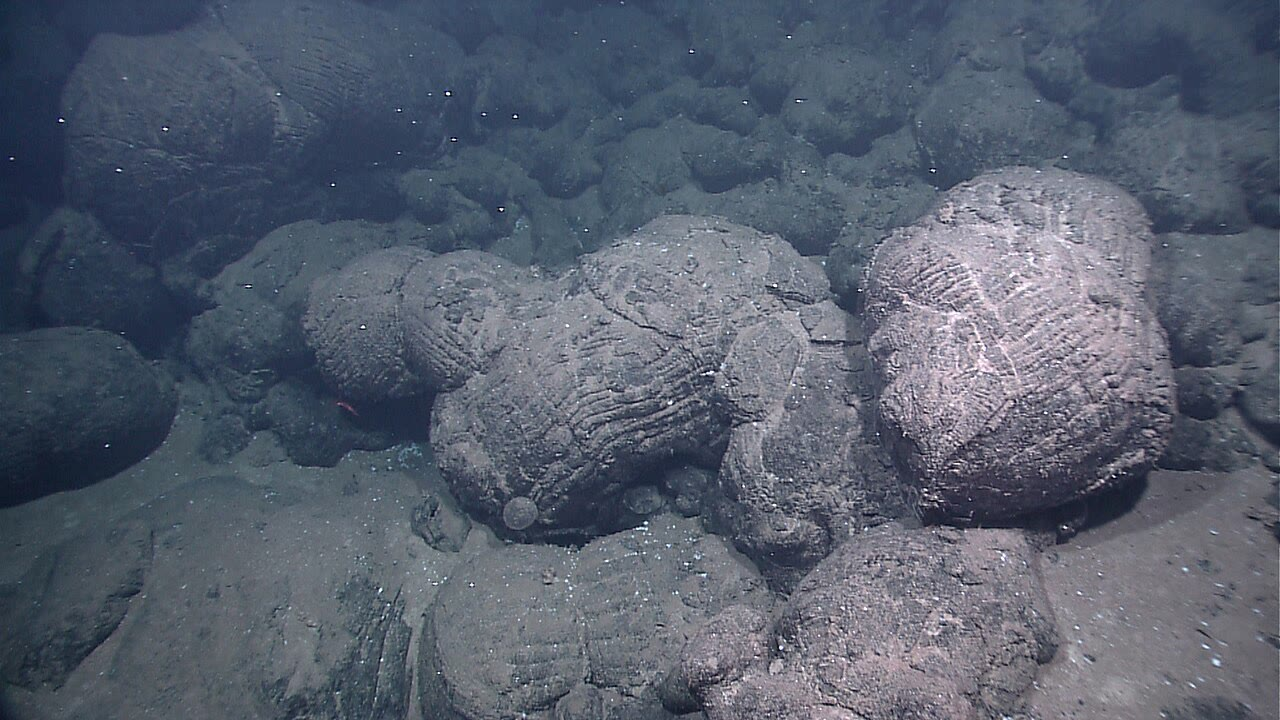
\includegraphics[width=0.8\linewidth]{images/book2/g11-noaa-pillow-lava.jpg}

{\small Laves en coussins sur le rift des Galápagos, vers 2500 mètres de
profondeur, photographiées par un robot téléguidé en 2011. Chaque coussin
est une langue de lave qui s'est figée de l'extérieur dès qu'elle a touché
l'eau de mer froide. Photographie~: NOAA Okeanos Explorer Program (domaine
public).}
\end{omfigure}
% ledger: photo:g11-pillow-lava, whoi:alvin-1977 (depth of the rift floor)

\section{Fondre sans chauffer}

Le manteau situé sous une dorsale est de la \omterm{def:g11:ocean-ridges:peridotite}{péridotite} solide, comme
partout ailleurs. Pourtant, \qty{7}{km} de basalte et de \omterm{def:g11:ocean-ridges:gabbro}{gabbro}, une roche
fondue qui s'est figée, en sont issus. D'où vient le liquide~?

\begin{definition}[Fusion partielle~; fusion par décompression]\label{def:g11:ocean-ridges:partial-melting}
La \emph{fusion partielle}\index{fusion partielle} est la fusion d'une
partie seulement d'une roche~: certains de ses minéraux, ou certains de
leurs constituants, fondent, tandis que le reste demeure solide. La
\emph{fusion par décompression}\index{fusion par decompression@fusion par décompression}
est la fusion partielle d'une roche qui remonte, et qui est
donc de moins en moins comprimée, sans être chauffée.
\end{definition}

Quand deux plaques s'écartent, l'\omterm{def:g11:lithosphere-asthenosphere:lithosphere}{asthénosphère} remonte sous la dorsale pour
combler le vide. Elle remonte trop vite pour perdre beaucoup de chaleur~:
sa température ne baisse donc que d'environ \qty{0.45}{\celsius} par
kilomètre pendant la remontée. Sa température de fusion, qui dépend de la
pression, baisse bien plus vite~: environ \qty{3.9}{\celsius} par kilomètre
à \qty{50}{km} de profondeur. À une certaine profondeur, la roche qui
remonte atteint sa température de fusion et commence à fondre, bien
qu'aucune chaleur n'ait été apportée.
% ledger: katsura10:adiabat, hirschmann:solidus, white92:crust; computed in
% figdata/grade-11/ridge_melting.py (solidus_slope_50km 3.89)

\begin{method}[Où le manteau qui remonte fond-il~?]\label{met:g11:ocean-ridges:melting}
\begin{enumerate}
  \item Écrire la température de la roche qui remonte à chaque
        profondeur~: sa température potentielle (la température qu'elle
        aurait en surface) plus \qty{0.45}{\celsius} par kilomètre de
        profondeur.
  \item Écrire la température de fusion de la roche à chaque profondeur, à
        partir de la pression à cette profondeur.
  \item Trouver la profondeur où les deux sont égales. Plus bas, la roche
        est solide~; plus haut, elle est partiellement fondue.
\end{enumerate}
\end{method}

\begin{omfigure}
\begin{tikzpicture}
\begin{axis}[omrecord, omdepth, width=0.72\linewidth, height=6.4cm, xmin=1100, xmax=1700, ymin=0, ymax=150,
  xlabel={température (\unit{\celsius})}, ylabel={profondeur (\unit{km})},
  xticklabel style={/pgf/number format/set thousands separator={}}, clip=true]
% computed in figdata/grade-11/ridge_melting.py; ledger: katsura10:adiabat, hirschmann:solidus, data:prem
\addplot[omProp, line width=1.0pt] table[x=solidus, y=z] {figdata/out/grade-11-ridge_melting-curves.dat};
\addplot[omDef, line width=1.0pt] table[x=ad1300, y=z] {figdata/out/grade-11-ridge_melting-curves.dat};
\addplot[omDef, densely dashed, line width=0.9pt] table[x=ad1400, y=z] {figdata/out/grade-11-ridge_melting-curves.dat};
\addplot[only marks, mark=*, mark size=1.8pt, black] coordinates {(1324.3,54.1) (1438.3,85.0)};
\node[font=\scriptsize, anchor=east, align=right] at (axis cs:1316,62) {début de la fusion,\\à \qty{54}{km}};
\node[font=\scriptsize, anchor=east] at (axis cs:1432,89) {\qty{85}{km}};
\node[font=\scriptsize, text=omProp, anchor=west, align=left] at (axis cs:1560,40) {température\\de fusion};
\node[font=\scriptsize, text=omDef, anchor=east, align=right] at (axis cs:1318,128) {manteau qui remonte,\\$T_p = \qty{1300}{\celsius}$};
\node[font=\scriptsize, text=omDef, anchor=west, align=left] at (axis cs:1476,140) {$T_p = \qty{1400}{\celsius}$};
\end{axis}
\end{tikzpicture}

{\small La température de la roche du manteau qui remonte sous une dorsale
(en bleu) et sa température de fusion (en orange), en fonction de la
profondeur. Une roche de température potentielle \qty{1300}{\celsius}
commence à fondre à \qty{54}{km} de profondeur~; une roche plus chaude de
\qty{100}{\celsius} (tirets) dès \qty{85}{km}. Température de fusion de la
\omterm{def:g11:ocean-ridges:peridotite}{péridotite} sèche d'après des expériences (Hirschmann, 2000).}
\end{omfigure}
% values: onset_1300_km 54.1, onset_1400_km 85.0, t_onset_1300 1324 (ridge_melting.py)

\begin{example}[La profondeur de la fusion]\label{ex:g11:ocean-ridges:onset}
Pour un manteau de température potentielle \qty{1300}{\celsius}, la roche
qui remonte est à $1300 + 0.45 \times 54 \approx \qty{1324}{\celsius}$
quand elle atteint \qty{54}{km}, exactement sa température de fusion à
cette profondeur~: la fusion commence vers \qty{54}{km} de profondeur.
Au-dessus de cette profondeur, la roche continue de fondre en remontant.
\end{example}

Seule une petite fraction de la \omterm{def:g11:ocean-ridges:peridotite}{péridotite} fond, et le liquide n'est pas de
la \omterm{def:g11:ocean-ridges:peridotite}{péridotite}~: c'est du basalte. Les liquides basaltiques se rassemblent
depuis toute la zone de fusion, qui s'étend de la profondeur de début de
fusion jusqu'à la base de la croûte~; plus légers que la roche solide qui
les entoure, ils montent jusqu'à l'axe de la dorsale. Là, une partie du
magma fait éruption sous forme de lave, une partie se fige en dykes dans les
fissures par lesquelles il est monté, et une partie cristallise lentement
plus bas sous forme de \omterm{def:g11:ocean-ridges:gabbro}{gabbro}. La \omterm{def:g11:ocean-ridges:peridotite}{péridotite} solide laissée sur place,
appauvrie de son basalte, devient la partie mantellique de la \omterm{def:g11:ocean-ridges:oceanic-lithosphere}{lithosphère
océanique}.
% ledger: asimow01:morb, geo:basalt-ridges, white92:crust

Là où une dorsale traverse une région de manteau plus chaud, autour d'un
point chaud, la fusion commence plus bas, une plus longue colonne de roche
fond et il se forme davantage de basalte~: la croûte y est épaisse
d'environ \qty{10}{km} au lieu de 7. À l'inverse, sous les dorsales très
lentes, le manteau qui remonte a le temps de perdre de la chaleur, fond
moins et forme une croûte exceptionnellement mince.
% ledger: white92:crust

\begin{omfigure}
\begin{tikzpicture}[font=\footnotesize]
  % schematic section across a ridge axis, not to scale
  \fill[omSea!45] (-6,0) rectangle (6,1.2);
  \fill[lith basalt] (-6,0) -- (-0.25,0) -- (-0.25,-0.35) -- (-6,-0.6) -- cycle;
  \fill[lith basalt] (6,0) -- (0.25,0) -- (0.25,-0.35) -- (6,-0.6) -- cycle;
  \fill[lith gabbro] (-6,-0.6) -- (-0.25,-0.35) -- (-0.25,-1.4) -- (-6,-1.6) -- cycle;
  \fill[lith gabbro] (6,-0.6) -- (0.25,-0.35) -- (0.25,-1.4) -- (6,-1.6) -- cycle;
  \fill[lith basalt] (-0.3,0) rectangle (0.3,-0.35);
  \fill[lith gabbro] (-0.3,-0.35) rectangle (0.3,-1.45);
  \fill[omProp!70] (-0.8,-0.75) .. controls (-0.4,-0.55) and (0.4,-0.55) .. (0.8,-0.75)
     .. controls (0.4,-0.95) and (-0.4,-0.95) .. (-0.8,-0.75);
  \fill[omProp!70] (-0.12,0) rectangle (0.12,-0.62);
  \fill[lith peridotite] (-6,-1.6) -- (-0.25,-1.4) -- (0.25,-1.4) -- (6,-1.6) -- (6,-5) -- (-6,-5) -- cycle;
  % melting region
  \fill[omProp!35] (-3.2,-1.5) -- (0,-4.0) -- (3.2,-1.5) -- cycle;
  \node[align=center] at (0,-2.95) {zone de fusion};
  % isotherms deepening away from the axis
  \draw[omDef!70!black, densely dashed] (-6,-2.6) .. controls (-2.5,-2.0) and (-1,-1.1) .. (0,-1.0) .. controls (1,-1.1) and (2.5,-2.0) .. (6,-2.6);
  \draw[omDef!70!black, densely dashed] (-6,-4.2) .. controls (-3,-3.6) and (-1.2,-2.0) .. (0,-1.9) .. controls (1.2,-2.0) and (3,-3.6) .. (6,-4.2);
  \node[text=omDef!70!black, anchor=west] at (6.05,-2.6) {\qty{800}{\celsius}};
  \node[text=omDef!70!black, anchor=west] at (6.05,-4.2) {\qty{1200}{\celsius}};
  % flow arrows
  \draw[-{Stealth[length=5pt]}, line width=0.9pt] (0,-4.9) -- (0,-4.2);
  \draw[-{Stealth[length=5pt]}, line width=0.9pt] (-1.2,-4.8) .. controls (-1.0,-3.8) and (-2.2,-3.2) .. (-3.6,-3.2);
  \draw[-{Stealth[length=5pt]}, line width=0.9pt] (1.2,-4.8) .. controls (1.0,-3.8) and (2.2,-3.2) .. (3.6,-3.2);
  \draw[-{Stealth[length=5pt]}, line width=1.1pt] (-2,0.6) -- (-4,0.6);
  \draw[-{Stealth[length=5pt]}, line width=1.1pt] (2,0.6) -- (4,0.6);
  \node[anchor=south] at (-3,0.65) {plaque};
  \node[anchor=south] at (3,0.65) {plaque};
  \node[anchor=west] at (1.0,-0.8) {lentille de magma};
  \node[anchor=east] at (-6.05,-0.3) {laves};
  \node[anchor=east] at (-6.05,-1.1) {gabbro};
  \node[anchor=east] at (-6.05,-3.3) {manteau};
  \node[anchor=north] at (0,-5.05) {le manteau remonte et fond};
\end{tikzpicture}

{\small Une coupe à travers l'axe d'une dorsale (schéma, sans échelle). Le
manteau remonte sous l'axe et fond partiellement~; le liquide se rassemble
dans une lentille de magma sous l'axe et construit la croûte, que les
plaques emportent des deux côtés. Les lignes d'égale température (tirets)
sont proches de la surface à l'axe et de plus en plus profondes à mesure
qu'on s'en éloigne~: la \omterm{def:g11:lithosphere-asthenosphere:lithosphere}{lithosphère} s'épaissit en refroidissant.}
\end{omfigure}

\section{Dorsales rapides et dorsales lentes}

Les dorsales s'ouvrent à des vitesses très différentes. D'après les pôles de
rotation du \cref{ch:g11:plate-motions}, la dorsale du Pacifique Est s'ouvre
à \ang{30} Sud à \qty{14.6}{cm} par an, la dorsale médio-atlantique à la
même latitude à \qty{3.3}{cm} par an. La forme de l'axe n'est pas la même.
% ledger: nnr56:poles (computed in plate_velocities.py: epr30s_speed 145.8, atl30s_speed 32.7)

Le long des dorsales lentes, l'axe est une vallée profonde de 1 à
\qty{2}{km} et large de 20 à \qty{30}{km}. Trop peu de magma atteint l'axe
pour combler le vide en continu~: la \omterm{def:g11:lithosphere-asthenosphere:lithosphere}{lithosphère} froide et cassante est
étirée et se rompt le long de failles.

\begin{definition}[Faille normale]\label{def:g11:ocean-ridges:normal-fault}
Une \emph{faille normale}\index{faille normale} est une faille inclinée le
long de laquelle le bloc situé au-dessus du plan de faille s'est abaissé
par rapport au bloc situé au-dessous. Les failles normales se forment là où
la croûte est étirée.
\end{definition}

La vallée d'une dorsale lente est un bloc qui s'est effondré entre des
\omterm{def:g11:ocean-ridges:normal-fault}{failles normales} qui se font face~; presque toutes plongent vers l'axe. Un
tel bloc effondré entre des \omterm{def:g11:ocean-ridges:normal-fault}{failles normales} s'appelle un \emph{graben} (ou
fossé d'effondrement).
% ledger: buck05:valley, usgs:normal-fault

Le long des dorsales rapides, le magma arrive assez souvent pour combler le
vide. L'axe est un bombement lisse et doux, au-dessus d'une lentille de
magma située dessous.
% ledger: buck05:valley, noaa:ridge

\begin{omfigure}
\begin{tikzpicture}[font=\footnotesize, x=0.24cm, y=0.9cm]
  % slow ridge: axial valley between normal faults (not to scale, vertical exaggeration)
  \begin{scope}
    \fill[omSea!45] (-15,-0.7) rectangle (15,1.6);
    \fill[lith basalt] (-15,0.9) -- (-9,0.9) -- (-8.5,0.2) -- (-6,0.2) -- (-5.5,-0.6) -- (5.5,-0.6)
      -- (6,0.2) -- (8.5,0.2) -- (9,0.9) -- (15,0.9) -- (15,-2.2) -- (-15,-2.2) -- cycle;
    \draw[black!70] (-15,0.9) -- (-9,0.9) -- (-8.5,0.2) -- (-6,0.2) -- (-5.5,-0.6) -- (5.5,-0.6)
      -- (6,0.2) -- (8.5,0.2) -- (9,0.9) -- (15,0.9);
    \draw[fault] (-9,0.9) -- (-7.4,-2.2);
    \draw[fault] (-6,0.2) -- (-4.6,-2.2);
    \draw[fault] (9,0.9) -- (7.4,-2.2);
    \draw[fault] (6,0.2) -- (4.6,-2.2);
    % slip arrows on the hanging walls (the axis side of each fault): down along the fault
    \foreach \x/\y/\s in {-7.9/-0.5/1, -5.0/-1.3/1, 7.9/-0.5/-1, 5.0/-1.3/-1} {
      \draw[-{Stealth[length=3pt]}, omProp, line width=0.8pt] (\x+0.9*\s,\y+0.45) -- ++(0.3*\s,-0.6);
    }
    \draw[-{Stealth[length=5pt]}, line width=1pt] (-11,1.25) -- (-14,1.25);
    \draw[-{Stealth[length=5pt]}, line width=1pt] (11,1.25) -- (14,1.25);
    \node at (0,-0.25) {vallée axiale};
    \node[anchor=north, align=center] at (0,-2.25) {dorsale lente~: une vallée\\entre des failles normales};
  \end{scope}
  % fast ridge
  \begin{scope}[xshift=8.2cm]
    \fill[omSea!45] (-15,0) rectangle (15,1.6);
    \fill[lith basalt] (-15,0.3) .. controls (-6,0.4) and (-2,0.9) .. (0,0.95) .. controls (2,0.9) and (6,0.4) .. (15,0.3)
      -- (15,-2.2) -- (-15,-2.2) -- cycle;
    \fill[omProp!75] (-2.5,-0.9) .. controls (-1,-0.7) and (1,-0.7) .. (2.5,-0.9) .. controls (1,-1.1) and (-1,-1.1) .. (-2.5,-0.9);
    \draw[black!70] (-15,0.3) .. controls (-6,0.4) and (-2,0.9) .. (0,0.95) .. controls (2,0.9) and (6,0.4) .. (15,0.3);
    \node[anchor=north] at (0,-1.25) {lentille de magma};
    \draw[-{Stealth[length=5pt]}, line width=1pt] (-8,1.25) -- (-14,1.25);
    \draw[-{Stealth[length=5pt]}, line width=1pt] (8,1.25) -- (14,1.25);
    \node at (0,1.3) {bombement axial};
    \node[anchor=north, align=center] at (0,-2.25) {dorsale rapide~: un bombement doux\\au-dessus d'une lentille de magma};
  \end{scope}
\end{tikzpicture}

{\small Coupes à travers une dorsale lente et une dorsale rapide (schémas,
sans échelle~; la hauteur est exagérée). À gauche~: la vallée axiale d'une
dorsale lente, profonde de 1 à \qty{2}{km}, s'est effondrée entre des
\omterm{def:g11:ocean-ridges:normal-fault}{failles normales} qui plongent vers l'axe (flèches orange~: les blocs situés
au-dessus des failles glissent vers le bas). À droite~: une dorsale rapide
s'élève doucement au-dessus d'une lentille de magma.}
\end{omfigure}
% ledger: buck05:valley

\begin{example}[Une dorsale lente et une dorsale rapide]\label{ex:g11:ocean-ridges:rates}
En un million d'années, la dorsale du Pacifique Est forme à \ang{30} Sud
$\qty{14.6}{cm/yr} \times 10^6\ \text{ans} = \qty{146}{km}$ de nouveau fond
océanique, \qty{73}{km} de chaque côté~; la dorsale médio-atlantique, à la
même latitude, en forme \qty{33}{km}, \qty{16.5}{km} de chaque côté. Le
forage profond du Pacifique Est a pénétré une croûte formée à plus de
\qty{20}{cm} par an, l'une des expansions les plus rapides jamais
enregistrées.
\end{example}
% ledger: nnr56:poles (computed), iodp1256:section

\section{Les sources hydrothermales}

La jeune croûte de l'axe est chaude, et elle est parcourue de fissures.
L'eau de mer s'y infiltre.

\begin{definition}[Circulation hydrothermale~; fumeur noir]\label{def:g11:ocean-ridges:hydrothermal}
La \emph{circulation hydrothermale}\index{circulation hydrothermale} est
l'écoulement de l'eau de mer qui descend par les fissures de la \omterm{def:g11:ocean-ridges:oceanic-lithosphere}{croûte
océanique} chaude, où elle est chauffée par le magma situé dessous et réagit
avec la roche, puis remonte jusqu'au fond marin, où elle ressort par des
\emph{sources hydrothermales}. Un \emph{fumeur noir}\index{fumeur noir} est
une source d'où jaillit une eau très chaude chargée de métaux dissous~; au
contact de l'eau de mer froide, des sulfures de fer et d'autres minéraux
précipitent en un nuage noir, et construisent une cheminée autour de la
source.
\end{definition}
% ledger: whoi:vents

L'eau d'un \omterm{def:g11:ocean-ridges:hydrothermal}{fumeur noir} sort en général de sa cheminée vers
\qty{350}{\celsius}, et les eaux des sources peuvent atteindre
\qty{400}{\celsius}. Elles ne bouillent pas, parce que deux kilomètres et
demi d'eau pèsent sur elles. Les cheminées peuvent dépasser \qty{10}{m} de
haut. Autour des sources, des bactéries tirent leur énergie du sulfure
d'hydrogène de l'eau des sources, et nourrissent des vers tubicoles, des
crevettes et des moules~: c'est de cela que vivaient les palourdes du rift
des Galápagos. La plupart des sources se trouvent le long des dorsales
médio-océaniques.
% ledger: whoi:vents, whoi:alvin-1977

\begin{omfigure}
\begin{minipage}[c]{0.6\linewidth}\centering
\begin{tikzpicture}[font=\scriptsize, x=0.8cm, y=0.62cm]
  \fill[omSea!45] (0,0) rectangle (10,3);
  \fill[lith basalt] (0,0) rectangle (10,-4);
  \fill[omProp!70] (2,-4.6) .. controls (4,-4.0) and (6,-4.0) .. (8,-4.6) -- (8,-5) -- (2,-5) -- cycle;
  \node at (5,-4.7) {magma};
  \fill[black!75] (4.7,0) -- (4.85,1.6) -- (5.15,1.6) -- (5.3,0) -- cycle;
  \fill[black!45, opacity=0.8] (5,1.7) circle (0.35) (5.2,2.2) circle (0.45) (4.9,2.7) circle (0.4);
  \draw[-{Stealth[length=4pt]}, omDef, line width=0.9pt] (1,0) .. controls (1,-2.5) and (2.5,-3.6) .. (4.2,-3.5);
  \draw[-{Stealth[length=4pt]}, omDef, line width=0.9pt] (9,0) .. controls (9,-2.5) and (7.5,-3.6) .. (5.8,-3.5);
  \draw[-{Stealth[length=4pt]}, omProp, line width=1.1pt] (5,-3.3) -- (5,-0.1);
  \node[align=center, text=omDef!80!black] at (1.6,1.0) {entrée d'eau\\de mer froide};
  \node[align=left, anchor=west] at (5.6,1.4) {fumeur noir,\\vers \qty{350}{\celsius}};
  \node[align=left, anchor=west, text=omProp!80!black, fill=white, fill opacity=0.85, text opacity=1, inner sep=1.5pt] at (5.3,-1.8) {chauffée,\\elle remonte};
\end{tikzpicture}
\end{minipage}\hfill
\begin{minipage}[c]{0.3\linewidth}\centering
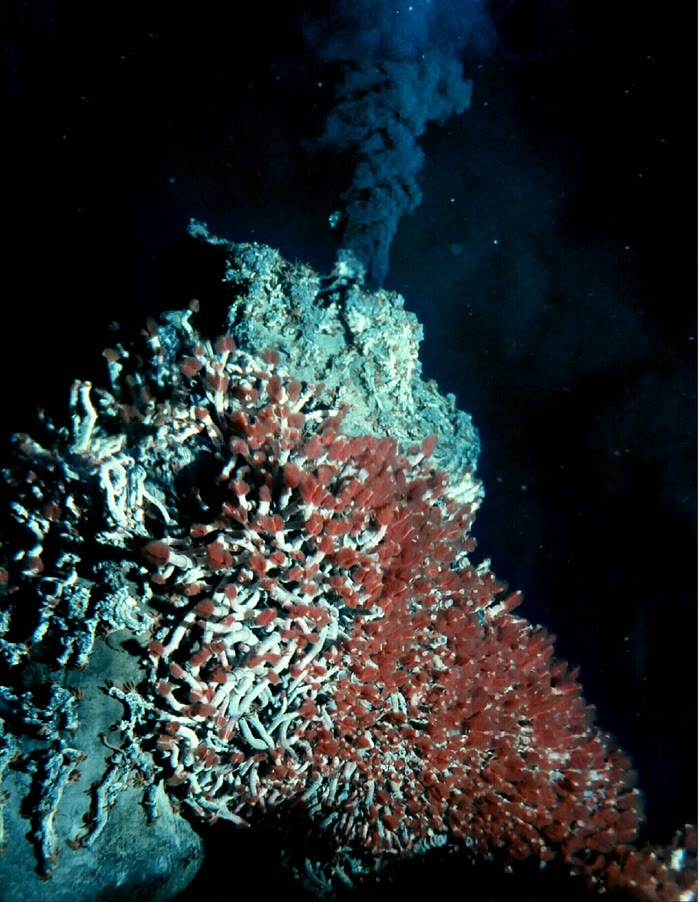
\includegraphics[width=\linewidth]{images/book2/g11-noaa-black-smoker.jpg}
\end{minipage}

{\small À gauche~: la \omterm{def:g11:ocean-ridges:hydrothermal}{circulation hydrothermale} à l'axe d'une dorsale
(schéma, sans échelle). À droite~: un \omterm{def:g11:ocean-ridges:hydrothermal}{fumeur noir} sur la dorsale Juan de
Fuca, dont la cheminée est couverte de vers tubicoles aux branchies
rouges~; photographie University of Washington et NOAA (domaine public).}
\end{omfigure}
% ledger: whoi:vents, photo:g11-black-smoker

\begin{history}[\emph{Alvin} sur le rift des Galápagos, 1977]
L'expédition, financée par la National Science Foundation, commença le
8~février 1977 à bord du navire de recherche \emph{Knorr}. Le traîneau
photographique ANGUS, remorqué à \qty{2500}{m} de profondeur au-dessus du
rift, enregistra une hausse de la température de l'eau, et sur les mêmes
images ses photographies montraient des centaines de palourdes blanches et
de coquilles de moules brunes sur la lave. Lors de la plongée~713
d'\emph{Alvin}, les géologues Jack Corliss et Tjeerd van Andel trouvèrent
une eau à \qty{8}{\celsius} qui sortait en miroitant des fissures, puis
jusqu'à \qty{17}{\celsius}, alors que l'eau profonde environnante était à
\qty{2}{\celsius}~; des palourdes blanches longues de \qty{30}{cm} au plus
couvraient une surface d'environ \qty{50}{m} de diamètre. Aucun biologiste
n'était à bord~: l'expédition était venue pour l'eau chaude, et trouva une
communauté d'animaux que personne n'avait imaginée.
\end{history}
% ledger: whoi:alvin-1977

\section{Refroidir, s'épaissir, s'enfoncer}

En s'éloignant de l'axe, la \omterm{def:g11:lithosphere-asthenosphere:lithosphere}{lithosphère} se refroidit par le haut, au
contact de l'océan froid qui la surmonte. La couche refroidie s'épaissit
avec le temps~: la \omterm{def:g11:lithosphere-asthenosphere:lithosphere}{lithosphère} s'épaissit, de quelques kilomètres à l'axe à
une centaine de kilomètres sous les fonds anciens. La roche refroidie se
contracte et devient plus dense~: la \omterm{def:g11:lithosphere-asthenosphere:lithosphere}{lithosphère} flotte donc plus bas sur
l'\omterm{def:g11:lithosphere-asthenosphere:lithosphere}{asthénosphère} (\omterm{def:g11:lithosphere-asthenosphere:isostasy}{isostasie}, \cref{ch:g11:lithosphere-asthenosphere}), et le
fond océanique s'enfonce en vieillissant. Pour un corps qui se refroidit
par conduction depuis sa surface, l'épaisseur de la couche refroidie croît
comme la racine carrée du temps.
% ledger: ps77:depth-age, rs09:lab

\begin{proposition}[Profondeur du fond océanique en fonction de son âge]\label{prop:g11:ocean-ridges:depth-age}
En moyenne, un fond océanique d'âge $t$ (en millions d'années) se trouve à
la profondeur
\[
  d(t) = 2500 + 350\sqrt{t} \quad \text{mètres} \qquad (0 \le t \le 70),
\]
et, pour un fond plus ancien qu'environ 20 millions d'années,
\[
  d(t) = 6400 - 3200\,e^{-t/62.8} \quad \text{mètres}:
\]
le fond s'enfonce vite tant qu'il est jeune, puis de plus en plus
lentement, vers environ \qty{6400}{m}. (Admis~: les formules ont été
ajustées aux profondeurs du Pacifique Nord et de l'Atlantique Nord,
corrigées du poids de leurs sédiments, par Parsons et Sclater en 1977.)
\end{proposition}
% ledger: ps77:depth-age

La racine carrée fait s'enfoncer vite le fond jeune~: pendant son premier
million d'années, le fond s'enfonce de \qty{350}{m}, pendant les trois
millions d'années suivants de \qty{350}{m} encore, et entre 16 et
64 millions d'années de \qty{1400}{m}, autant que pendant ses seize premiers
millions d'années. La loi exponentielle décrit la façon dont le fond ancien
cesse de s'enfoncer~: il se comporte comme si la plaque qui se refroidit
avait une épaisseur fixe, d'environ \qty{125}{km}.
% ledger: ps77:depth-age

\begin{omfigure}
\begin{tikzpicture}
\begin{axis}[omrecord, omdepth, width=0.82\linewidth, height=6.2cm, xmin=0, xmax=180, ymin=2000, ymax=6600,
  xlabel={âge du fond océanique (millions d'années)}, ylabel={profondeur (\unit{m})},
  yticklabel style={/pgf/number format/set thousands separator={}},
  legend style={font=\scriptsize, at={(0.5,-0.32)}, anchor=north, legend columns=3, /tikz/every even column/.append style={column sep=6pt}}, legend cell align=left]
% computed in figdata/grade-11/depth_age.py; ledger: data:etopo1, data:b2-seafloor-age, ps77:depth-age
\addplot[only marks, mark=*, mark size=1.3pt, black!70, error bars/.cd, y dir=both, y explicit]
  table[x=age, y=depth, y error minus=em, y error plus=ep] {figdata/out/grade-11-depth_age-bins.dat};
\addplot[omProp, line width=1.0pt] table[x=age, y=depth] {figdata/out/grade-11-depth_age-sqrt.dat};
\addplot[omDef, line width=1.0pt, densely dashed] table[x=age, y=depth] {figdata/out/grade-11-depth_age-exp.dat};
\legend{{mesures~: médiane et moitié centrale}, {$2500 + 350\sqrt{t}$}, {$6400 - 3200\,e^{-t/62.8}$}}
\end{axis}
\end{tikzpicture}

{\small Profondeur du fond océanique en fonction de son âge~: pour chaque
tranche d'âge de 5 millions d'années, la profondeur médiane de toutes les
cellules d'un degré des océans du monde, et l'étendue de la moitié centrale
d'entre elles. Le fond jeune suit de près la loi en racine carrée~; le fond
plus ancien est moins profond que les lois, parce que ses cellules
comprennent des sédiments et des volcans. Données~: ETOPO1 (NOAA) et les
âges du fond océanique de Seton et de ses collègues (2020)~; lois de
Parsons et Sclater (1977).}
\end{omfigure}
% values (depth_age.py): median 2.5-5 Myr 3114 (law 3178), 60-65 Myr 4648 (law 5267), fit a 2727 b 255

Les profondeurs mesurées du fond jeune concordent avec la loi à environ
\qty{100}{m} près. Sur les fonds plus anciens, les médianes mesurées se
trouvent plusieurs centaines de mètres au-dessus des lois. Les lois
décrivent la profondeur du fond lui-même, comme si ses sédiments étaient
retirés~; les cellules mesurées portent encore leurs sédiments, qui
s'épaississent avec l'âge du fond et dépassent un kilomètre d'épaisseur sur
les fonds les plus anciens de l'ouest de l'Atlantique Nord, et elles
comprennent des monts sous-marins et des plateaux volcaniques.
% ledger: ps77:depth-age; values from depth_age.py

La \omterm{def:g11:ocean-ridges:oceanic-lithosphere}{lithosphère océanique} ancienne est donc épaisse, froide et dense. Le
chapitre suivant montre qu'elle peut devenir plus dense que l'\omterm{def:g11:lithosphere-asthenosphere:lithosphere}{asthénosphère}
située dessous, et replonger dans le manteau (\cref{ch:g11:subduction-zones}).

\section{Exercices}

\begin{exercise}[$\star$]\label{exo:g11:ocean-ridges:1}
Définir la \omterm{def:g11:ocean-ridges:peridotite}{péridotite} et le \omterm{def:g11:ocean-ridges:gabbro}{gabbro}. Lequel des deux appartient à la \omterm{def:g11:ocean-ridges:oceanic-lithosphere}{croûte
océanique}, et lequel au manteau~? Le \omterm{def:g11:ocean-ridges:gabbro}{gabbro} a la même composition que le
basalte~: pourquoi ses cristaux sont-ils tellement plus grands~?
\end{exercise}

\begin{exercise}[$\star$]\label{exo:g11:ocean-ridges:2}
Énumérer les couches de la \omterm{def:g11:ocean-ridges:oceanic-lithosphere}{lithosphère océanique} depuis le fond marin vers
le bas. Le forage profond du Pacifique Est a atteint \qty{1507}{m} sous le
fond marin~: quelle fraction d'une croûte de \qty{7.1}{km} a-t-il
traversée~?
\end{exercise}

\begin{exercise}[$\star$]\label{exo:g11:ocean-ridges:3}
À l'aide de $d = 2500 + 350\sqrt{t}$, trouver la profondeur d'un fond
océanique âgé de 0, 9 et 25 millions d'années.
\end{exercise}

\begin{exercise}[$\star$]\label{exo:g11:ocean-ridges:4}
Définir une \omterm{def:g11:ocean-ridges:normal-fault}{faille normale}. À une dorsale lente, quelle force produit les
\omterm{def:g11:ocean-ridges:normal-fault}{failles normales}, et dans quelle direction se déplacent les blocs situés
au-dessus des failles~?
\end{exercise}

\begin{exercise}[$\star$]\label{exo:g11:ocean-ridges:5}
L'eau d'un \omterm{def:g11:ocean-ridges:hydrothermal}{fumeur noir} sort vers \qty{350}{\celsius}. Pourquoi ne bout-elle
pas~? Qu'est-ce que la «~fumée~» noire~?
\end{exercise}

\begin{exercise}[$\star\star$]\label{exo:g11:ocean-ridges:6}
À l'aide de la figure de la fusion~: (1) à quelle profondeur un manteau de
température potentielle \qty{1300}{\celsius} commence-t-il à fondre, et à
quelle température~? (2) Et un manteau plus chaud de \qty{100}{\celsius}~?
(3) Lequel des deux forme la croûte la plus épaisse~? Pourquoi~?
\end{exercise}

\begin{exercise}[$\star\star$]\label{exo:g11:ocean-ridges:7}
Une roche du manteau qui remonte, de température potentielle
\qty{1300}{\celsius}, est à \qty{1345}{\celsius} à \qty{100}{km} de
profondeur, où sa température de fusion vaut \qty{1489}{\celsius}. (1) De
combien est-elle sous sa température de fusion~? (2) Elle commence à fondre
à \qty{54}{km}. De combien de degrés par kilomètre, en moyenne, l'écart
s'est-il réduit pendant la remontée~? (3) La roche a-t-elle été chauffée~?
\end{exercise}

\begin{exercise}[$\star\star$]\label{exo:g11:ocean-ridges:8}
La dorsale du Pacifique Est s'ouvre à \qty{14.6}{cm} par an à \ang{30} Sud,
la dorsale médio-atlantique à \qty{3.3}{cm} par an. En supposant
l'expansion symétrique, combien de temps chaque dorsale met-elle pour
former \qty{1000}{km} de fond d'un côté~?
\end{exercise}

\begin{exercise}[$\star\star$]\label{exo:g11:ocean-ridges:9}
Les dorsales ont une longueur d'environ \qty{65000}{km}. Supposons qu'elles
s'ouvrent en moyenne à \qty{5}{cm} par an et forment une croûte épaisse de
\qty{7.1}{km}. (1) Quelle surface de nouveau fond océanique forment-elles
chaque année~? (2) Quel volume de croûte~? (3) Combien de temps
mettraient-elles pour former une surface égale à celle des océans,
\qty{3.6e8}{km^2}~?
\end{exercise}

\begin{exercise}[$\star\star$]\label{exo:g11:ocean-ridges:10}
Une vallée axiale est profonde de \qty{1.5}{km}. Elle s'est effondrée le
long de deux \omterm{def:g11:ocean-ridges:normal-fault}{failles normales} qui se font face, plongeant chacune de
\ang{60}. (1) De combien chaque faille a-t-elle joué le long de son plan~?
(2) De combien les deux bords se sont-ils écartés horizontalement du fait
des deux failles~? (3) La vallée est large de \qty{25}{km}~: le jeu des
failles l'a-t-il formée à lui seul~?
\end{exercise}

\begin{exercise}[$\star\star$]\label{exo:g11:ocean-ridges:11}
À l'aide de $d = 6400 - 3200\,e^{-t/62.8}$, trouver la profondeur d'un fond
âgé de 25 et de 100 millions d'années, et de combien le fond s'enfonce entre
ces âges. Comparer la première valeur à celle de la loi en racine carrée.
\end{exercise}

\begin{exercise}[$\star\star\star$]\label{exo:g11:ocean-ridges:12}
Une colonne de manteau épaisse de \qty{100}{km} se refroidit en moyenne de
\qty{700}{\celsius}. La roche se contracte de $\alpha = 3.2 \times 10^{-5}$
de sa longueur par degré de refroidissement. (1) De combien la colonne
raccourcit-elle~? (2) À mesure qu'elle s'enfonce, l'eau de mer
(\qty{1025}{kg/m^3}) remplit l'espace situé au-dessus~; avec une masse
volumique du manteau de \qty{3380}{kg/m^3}, l'\omterm{def:g11:lithosphere-asthenosphere:isostasy}{isostasie} fait s'enfoncer le
fond de $s = \rho_m\,\alpha\,\Delta T\,L/(\rho_m - \rho_w)$. Calculer $s$.
(3) Comparer à l'enfoncement total que permet la loi exponentielle, de
\qty{2500}{m} à \qty{6400}{m}.
\end{exercise}

\begin{exercise}[$\star\star\star$]\label{exo:g11:ocean-ridges:13}
La fusion commence à \qty{54}{km} de profondeur dans un manteau à
\qty{1300}{\celsius}, à \qty{85}{km} dans un manteau à \qty{1400}{\celsius}~;
dans les deux, la fusion se poursuit jusqu'à la base de la croûte, vers
\qty{7}{km} de profondeur. (1) Comparer les longueurs des deux colonnes de
fusion. (2) Si chaque kilomètre de roche qui remonte donnait la même
quantité de liquide, quelle serait l'épaisseur de la croûte au-dessus du
manteau le plus chaud, pour une croûte de \qty{7.1}{km} au-dessus du
manteau normal~? (3) Comparer aux \qty{10.3}{km} mesurés là où les dorsales
rencontrent un manteau plus chaud.
\end{exercise}

\begin{exercise}[$\star\star\star$]\label{exo:g11:ocean-ridges:14}
Les profondeurs médianes mesurées du fond océanique valent \qty{3114}{m} à
l'âge de \num{3.75} millions d'années, \qty{4018}{m} à \num{22.5},
\qty{4465}{m} à \num{42.5} et \qty{4648}{m} à \num{62.5}. (1) Calculer la
profondeur donnée par la loi en racine carrée à chaque âge, et l'écart avec
la mesure. (2) Comment l'écart varie-t-il avec l'âge~? (3) L'expliquer.
\end{exercise}

\begin{exercise}[$\star\star\star$]\label{exo:g11:ocean-ridges:15}
Le point critique de l'eau se situe à \qty{374}{\celsius} et
\qty{22.064}{MPa}~: au-dessus de cette pression, l'eau ne bout à aucune
température. (1) Calculer la pression de l'eau à \qty{2500}{m} de
profondeur (eau de mer à \qty{1025}{kg/m^3}, $g = \qty{9.8}{m/s^2}$, plus
les \qty{0.1}{MPa} de l'atmosphère). (2) L'eau d'une source peut-elle
bouillir à cette profondeur, quelle que soit sa température~? (3) Au-delà
d'environ quelle profondeur est-ce vrai pour toutes les sources~?
\end{exercise}

\section{Problème~: la vie d'un morceau de fond du Pacifique}

\begin{problem}[{Problème du week-end --- de la dorsale à l'océan profond}]
\label{pb:g11:ocean-ridges:1}
% values: EPR 30 S full rate 145.8 mm/yr (plate_velocities.py, nnr56:poles); depth law
% ps77:depth-age; crust white92:crust; alpha ps77; densities data:prem; median 60-65 Myr
% 4648 m (depth_age.py)
Un morceau de fond océanique naît aujourd'hui sur la dorsale du Pacifique
Est à \ang{30} Sud, où les plaques Pacifique et de Nazca s'écartent de
\qty{14.6}{cm} par an. Il se déplace vers l'ouest avec la plaque Pacifique.
On prend l'expansion symétrique, la croûte épaisse de \qty{7.1}{km}, et la
loi de profondeur $d = 2500 + 350\sqrt{t}$ mètres ($t$ en millions
d'années).

\medskip
\noindent\textbf{Partie I --- La naissance à la dorsale.}
\begin{enumerate}
  \item Quelle est la demi-vitesse d'expansion, en centimètres par an et en
        kilomètres par million d'années~?
  \item À quelle profondeur le morceau de fond naît-il~?
  \item Énumérer les roches qui le composent, depuis le fond marin jusqu'à
        la base de la \omterm{def:g11:lithosphere-asthenosphere:lithosphere}{lithosphère}.
  \item Le magma qui l'a formé venait du manteau situé dessous. Expliquer
        comment le manteau a fondu sans être chauffé.
  \item Quel volume de croûte cette dorsale forme-t-elle chaque million
        d'années, des deux côtés, pour chaque kilomètre de sa longueur~?
\end{enumerate}

\medskip
\noindent\textbf{Partie II --- Le voyage.}
\begin{enumerate}[resume]
  \item À quelle distance de la dorsale le morceau se trouvera-t-il au bout
        de 1, 4, 16 et 64 millions d'années, si la vitesse reste la même~?
  \item Combien de temps mettra-t-il pour parcourir \qty{2000}{km}~?
  \item Pourquoi la distance réelle au bout de 64 millions d'années
        peut-elle différer de la réponse à la question~6~?
  \item Près de la dorsale, l'eau de mer circule à travers la jeune croûte
        et ressort par des sources. Pourquoi cette circulation cesse-t-elle
        sur les fonds anciens~?
  \item Sur quelle plaque le morceau voyage-t-il, et vers quel type de
        limite de plaques cette plaque l'emporte-t-elle, sur son côté
        ouest~?
\end{enumerate}

\medskip
\noindent\textbf{Partie III --- S'enfoncer en vieillissant.}
\begin{enumerate}[resume]
  \item Calculer sa profondeur à 1, 4, 16 et 64 millions d'années.
  \item De combien s'enfonce-t-il pendant ses 16 premiers millions
        d'années, et entre 16 et 64 millions d'années~? Commenter.
  \item À quel âge atteint-il une profondeur de \qty{4000}{m}~?
  \item Comparer sa profondeur à 64 millions d'années à la loi
        exponentielle, $6400 - 3200\,e^{-t/62.8}$.
  \item La profondeur médiane mesurée des fonds océaniques âgés de 60 à
        65 millions d'années est de \qty{4648}{m}. Expliquer la différence.
\end{enumerate}

\medskip
\noindent\textbf{Partie IV --- Sa masse volumique et son destin.}
\begin{enumerate}[resume]
  \item À 64 millions d'années, prendre sa \omterm{def:g11:lithosphere-asthenosphere:lithosphere}{lithosphère} épaisse de
        \qty{100}{km} et en moyenne plus froide de \qty{700}{\celsius} que
        l'\omterm{def:g11:lithosphere-asthenosphere:lithosphere}{asthénosphère}. Avec $\alpha = 3.2 \times 10^{-5}$ par degré, de
        quelle fraction la partie mantellique est-elle devenue plus
        dense~? En partant de \qty{3380}{kg/m^3}, quelle est sa masse
        volumique~?
  \item Sa croûte est épaisse de \qty{7.1}{km}, avec une masse volumique de
        \qty{2900}{kg/m^3}. Calculer la masse volumique moyenne de
        l'ensemble des \qty{100}{km} de \omterm{def:g11:lithosphere-asthenosphere:lithosphere}{lithosphère}.
  \item La comparer à celle de l'\omterm{def:g11:lithosphere-asthenosphere:lithosphere}{asthénosphère} située dessous, prise à
        \qty{3380}{kg/m^3}.
  \item Que peut faire une telle \omterm{def:g11:lithosphere-asthenosphere:lithosphere}{lithosphère} quand elle atteint une
        fosse~?
  \item Conclure~: à quelle profondeur se trouve ce morceau de fond quand
        il a 64 millions d'années~?
\end{enumerate}
\end{problem}
